%\documentclass[notes=show]{beamer}
\documentclass{beamer}
%\usefonttheme{professionalfonts} % using non standard fonts for beamer
%\usepackage[T1]{fontenc}
%\usepackage[utf8]{inputenc}
%\usepackage{mathptmx} % doesn't work?

\usepackage{graphicx} 
\usepackage{amsmath}
\usepackage{amsthm}
\usepackage{amssymb}
\usepackage{bm}
\usepackage{bbm}
\usepackage{lipsum}
\usepackage{ulem}
\usepackage{tikz}
\usepackage{fancyvrb}

\newcommand{\iter}[2]{#1^{(#2)}{}}
\newcommand{\ra}{\rightarrow}
\newcommand{\la}{\leftarrow}
\newcommand{\lra}{\Leftrightarrow}

\newcommand{\bmat}{\left[\begin{matrix}}
\newcommand{\emat}{\end{matrix}\right]}

\newcommand{\norm}[1]{\left\lVert#1\right\rVert}
\newcommand{\param}[1]{\left(#1\right)}
\newcommand{\set}[1]{\left\{#1\right\}}
\newcommand{\vect}[1]{\left<#1\right>}
\newcommand{\arr}[1]{\left[#1\right]}
\newcommand{\ceil}[1]{\left\lceil{ #1 }\right\rceil}
\newcommand{\floor}[1]{\left\lfloor{ #1 }\right\rfloor}

\newcommand{\inv}{^{-1}}

\newcommand{\maximize}[1]{\underset{#1}{\mathrm{maximize}\;}}
\newcommand{\argmin}[1]{\underset{#1}{\mathrm{argmin}\;}}

% Text
\newcommand{\range}{\textbf{range}}
\newcommand{\Sup}{\text{Sup}}
\newcommand{\Inf}{\text{Inf}}
\newcommand{\Mod}{\text{Mod}}
\newcommand{\dual}{\text{dual}}
\newcommand{\prop}{\text{prop}}
\newcommand{\wid}{\text{wid}}
\newcommand{\iftext}{\text{ if }}

% Operations
\newcommand{\Oh}{\mathcal O}

% Algebras
\newcommand{\Reals}{\mathbb R}
\newcommand{\Naturals}{\mathbb N}
\newcommand{\Field}{\mathbb{F}}
\newcommand{\Integers}{\mathbb{Z}}
\newcommand{\Rationals}{\mathbb{Q}}
\newcommand{\Complex}{\mathbb{C}}
\newcommand{\Kaucher}{\mathbb{KR}}
\newcommand{\RIntervals}{\mathbb{IR}}

% Sets
\newcommand{\cP}{\mathcal P}
\newcommand{\cI}{\mathcal I}

\graphicspath{ {.} }

\renewcommand{\iter}[1]{^{(#1)}}
\newcommand{\iterx}[1]{\bm{x}^{(#1)}}
\newcommand{\itertx}[1]{\tilde{\bm{x}}^{(#1)}}
\newcommand{\iterJ}[1]{J^{(#1)}}
\newcommand{\layf}[1]{\bm{f}^{[#1]}}
\newcommand{\layJ}[1]{\text{Jac}_z \bm{f}^{[#1]}}
\newcommand{\autof}[1]{\bm{f}^{[#1]}}
\newcommand{\fMV}{f^{\text{MV}}}

\newcommand{\intervalbox}[1]{\arr{\bm{x}^{(#1)}}}
\newcommand{\tintervalbox}[1]{\arr{\tilde{\bm{x}}^{(#1)}}}
\newcommand{\Intervalbox}[1]{\arr{J^{(#1)}}}

\newcommand{\enclosure}[1]{\arr{\bm{r}^{(#1)}}}
\newcommand{\tenclosure}[1]{\arr{\tilde{\bm{r}}^{(#1)}}}
\newcommand{\Jac}[1]{\text{Jac}_{#1}}
\newcommand{\Enclosure}[1]{\arr{R^{(#1)}}}

\title{Reachability of Non-Linear Continuous Systems}
\author{Colin Chen}

\begin{document}

\begin{frame}
    \titlepage
\end{frame}

\begin{frame}
    \frametitle{Reachability of Non-Linear Continuous Systems}

    Eric Goubault and Sylvie Putot (French Alternative Energies and Atomic Energy Commission (CEA))
    \textit{Forward Inner-Approximated Reachability of Non-Linear Continuous Systems} (HSCC 2017)
\end{frame}

\note{
    Today I'll be presenting my contributions towards the Reachability of Non-Linear Continuous Systems.
Part of this presentation will be for me to flesh out what I skipped over last presentation.
But I'll also be talking about my software implementation of the algorithm in this paper.
}

\begin{frame}
    \frametitle{Problem}

    Problem specification:

    a system of first order autonomous ODEs $\dot{\bm{x}} = \bm{f}(\bm{x})$ where $\bm{f}: \Reals^n \ra \Reals^n$, 
    a time interval $[t_0, t_n]$ and initial conditions $\intervalbox{0} \in \RIntervals$.
    \par We assume $\bm{f}$ is infinitely differentiable.

    \vspace{7mm}
    Definitions:

    Suppose $\bm{x}(t, t_0, \iterx{0})$ represents a solution to the ODE.
    \par Fix $t \in [t_0, t_n]$.
    \par $\range_t(\bm{x}, \intervalbox{0}) = \bm{x}(t, t_0, \intervalbox{0})$
    is the set of all possible values $\bm{x}(t, t_0, \iterx{0})$ at $t$ given an initial conditions $\iterx{0} \in \intervalbox{0}$.

\end{frame}

\note{
The problem presented in Goubault and Putot's paper centers around systems of autonomous ODEs.
Note all forms of higher order autonomous ODEs can be converted to this system form. 
This seems like a set up to a initial value problem (IVP) except we have a range of initial conditions instead of one point.

$\intervalbox{0}$ is the range of initial inputs. It is represented by a vector of intervals. You can tell because it is bolded and has square brackets.

If we fix $t \in [t_0, t_n]$ then the set of $\bm{x}$ ($\range(\bm{x}, \intervalbox{0}) = \bm{x}(t, t_0, \intervalbox{0})$)
represents all possible solutions 
is the range of all possible values $\bm{x}(t, t_0, x_0)$ with initial conditions $x_0$ is $\intervalbox{0}$
}

\begin{frame}
    \frametitle{Problem}

    $\bigcup_{t \in [t_0, t_n]} \range_t(\bm{x}, \intervalbox{0})$ is our \emph{reachable state} or \emph{flowpipe}.

    \vspace{7mm}
    At each slice of time...
    \begin{itemize}
        \item Outer approximations $[\bm{x}]$:
        \begin{itemize}
            \item $\range_t(\bm{x}, \intervalbox{0}) \subseteq [\bm{x}](t, t_0, x_0)$
        \end{itemize}
        \vspace{3mm}
        \item Inner approximations $]\bm{x}[$:
            \begin{itemize}
                \item $]\bm{x}[(t, t_0, x_0) \subseteq \range_t(\bm{x}, \intervalbox{0})$
            \end{itemize}
    \end{itemize}

\end{frame}

\note{
    Draw a picture.
}

\begin{frame}
    \frametitle{Problem}

    Goal:
    Find tight inner and outer approximations of reachable states for all initial conditions in $\intervalbox{0}$ over time interval $[t_0, t_n]$.
\end{frame}

\begin{frame}
    \frametitle{Outcome}

    Results can be used to solve other kinds of problems.

    \vspace{5mm}
    Dynamical systems with inputs $t \in \Reals^+_0, u \in \set{\phi : \Reals^+_0 \ra \Reals^m}$:
    $$\dot{x}(t) = \begin{cases} 
        f(x(t), u(t)) & \text{ if } t \geq 0\\
        z_0 & \text{ if } t = 0\\
    \end{cases}$$

    Delayed Differential Equations with inputs $t \in \Reals^+_0$
    \par and fixed parameters $\beta \in \Reals^m$
    $$\begin{cases}
        \dot{x}(t) = f(x(t), x(t-\tau), \beta) & \iftext t \geq t_0+\tau \\
            x(t) = x_0(t, \beta) & \iftext t \in [t_0, t_0+\tau] \\
    \end{cases}$$

\end{frame}

\note{
    It's good to remind ourselves why we are working on certain problems. Being able to find an algorithm to find inner/outer approx. of ODEs opens doors to tweaks of the algorithm to solve similar kinds of problems.
    Obtaining inner/outer approx. for dynamical systems allows use to work on safety problems to find minimal/maximal reachable sets.
    
Obtaining inner/outer approx. of DDEs allows us to approximate equations that are hard to solve due to inital conditions being a functional instead of a value.

These problems are mentioned in Goubault and Putot's followup papers (HSCC'18 and HSCC'19)
}

\begin{frame}
    \frametitle{Solution}

    What I made:

    \vspace{5mm}
    \begin{enumerate}
        \item Flowpipes.jl
        \item AffineArithmetic.jl (better intervals)
        \item ModalIntervalArithmetic.jl
    \end{enumerate}

    \vspace{5mm}
    Bonus: hacked ForwardDiff.jl

    \vspace{5mm}
    Based on:

    {\small
RINO \quad \url{https://github.com/cosynus-lix/RINO}

aaflib \quad \url{http://aaflib.sourceforge.net}

Miguel A. Sainz et al. - \textit{Modal Interval Analysis: New Tools for Numerical Information} (Lecture Notes in Mathematics, Springer 2014)
}

\end{frame}

\note{
    This Summer I spent my time working on the solution to the algorithm. I ended up completing three components.

Flowpipes.jl implements the algorithm in Goubault and Putot's paper to compute tight inner and outer approx. of reachable states for a set of initial conditions over a time interval.

ForwardDiff.jl is a reimplementation of another software: RINO (Robust INner and Outer approximated reachability analysis) written in C++ by the authors. RINO is a demonstration, not a numerical computing solver so I wanted to turn it into a usable solver.

AffineArithmetic.jl is mainly used to limit catastropic overestimation in interval arithmetic. Affine forms are also what RINO uses.

ModalIntervalArithmetic.jl is uses the algorithms in the Modal Interval Analysis book to construct the modal interval type and it's operations.
}

\begin{frame}
    \frametitle{Solution: AffineArithmetic.jl}

    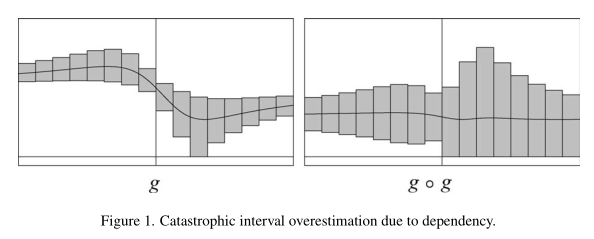
\includegraphics[width=1.0\textwidth]{overestimate.png}
    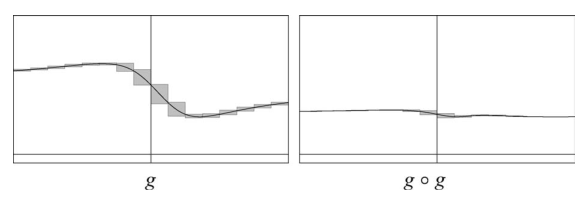
\includegraphics[width=1.0\textwidth]{good.png}

\end{frame}

\begin{frame}
    \frametitle{Solution: Flowpipes.jl algorithm}

    Discretize $t_0 < t_1 < \cdots < t_j < t_{j+1} = t_j + \tau < \cdots < t_n$

\end{frame}

\note{
RINO does not use a library for modal intervals. Instead RINO use very many if-else conditionals to check whether the endpoints of the intervals were proper/improper.

The pre-existing packages / features in RINO and associated libraries were non-existant for Julia so I ended up building almost everything from scratch.
This includes the half features of the C++ automatic diff. software (FADBAD++) because Julia does not have a library that calculates some kinds of taylor coefficients (will see in a moment).

To use a numerical method solution we just discretize time and find the approx. at each time step.
}

\begin{frame}
    \frametitle{Solution: Flowpipes.jl algorithm}

    Discretize $t_0 < t_1 < \cdots < t_j < t_{j+1} = t_j + \tau < \cdots < t_n$

    %Let $\tintervalbox{0} := \text{mid}\intervalbox{0}$

    \vspace{3mm}
    For each $j = 0,\ldots,n$
    \begin{enumerate}
        \item get priori enclosure of
        \begin{itemize}
            \item $\enclosure{j+1}$ of \; $\bm{x}(t, t_j, \intervalbox{j})$
            \item $\tenclosure{j+1}$ of \; $\bm{x}(t, t_j, \tintervalbox{j})$
            \item $\Enclosure{j+1}$ of \; $J(t, t_j, \intervalbox{j}) = \Jac{\iterx{j}} \bm{x}(t, t_j, \intervalbox{j})$
        \end{itemize}
        over $t \in [t_j, t_{j+1}]$

        \vspace{3mm}
    \item get taylor approximations $[\bm{x}](t_{j+1}, t_j, \intervalbox{j})$, $[\bm{x}](t_{j+1}, t_j, \tintervalbox{j})$ and $[J](t_{j+1}, t_j, \intervalbox{j})$

        \vspace{3mm}
    \item deduce an inner approximation $]\bm{x}[(t_{j+1}, t_j, \intervalbox{j})$

        \vspace{3mm}
        \item set $]\iterx{j+1}[$, $\intervalbox{j+1}, \tintervalbox{j+1}$ and $\Intervalbox{j+1}$
    \end{enumerate}

\end{frame}

\note{
The authors Goubault and Putot did not really walk the readers through the proof of their algorithm in the paper.

Since I'm likely to write up a documentation for the software I thought I would go over each step with new details and provide some illustrative examples.

The algorithm has 3 steps with the purpose of acquiring the outer bounds listing in step 4 for each iteration $j$.


This is a high level of what we're doing.
Draw a picture.

Remember, the $\bm{x}$ refers to the actual range of the solution at $t$, $[\bm{x}]$ are outer approximation of that range, and $]\bm{x}[$ are the inner approximation of that range.

Priori enclosures outer bound of the actual range $\bm{x}$ for all values $t \in [t_j, t_{j+1}]$.
}

\begin{frame}
    \frametitle{Step 0: initialize data}

    Discretization $t_0 < t_1 < \cdots < t_j < t_{j+1} = t_j + \tau < \cdots < t_n$

    \vspace{3mm}
    Outer approximation $[\iterx{0}]$ (given)

    \vspace{3mm}
    Outer approximation $[\iterJ{0}] := I$

    \vspace{3mm}
    Outer approximate center of $[\iterx{0}]$ as $[\itertx{0}] := \text{mid}{\intervalbox{0}}$

    \vspace{3mm}
    Inner approximation $]\iterx{0}[ = [\iterx{0}]$

\end{frame}

\begin{frame}
    \frametitle{Step 1: for each $j = 1,\ldots$, priori enclosures}
    
    Get priori enclosure of
    \begin{itemize}
        \item $\enclosure{j+1}$ of \; $\bm{x}(t, t_j, \intervalbox{j})$
        \item $\tenclosure{j+1}$ of \; $\bm{x}(t, t_j, \tintervalbox{j})$
        \item $\Enclosure{j+1}$ of \; $J(t, t_j, \intervalbox{j}) = \Jac{\iterx{j}} \bm{x}(t, t_j, \intervalbox{j})$
    \end{itemize}
    over $t \in [t_j, t_{j+1}]$

\end{frame}

\note{
Priori enclosures outer bound of the actual range $\bm{x}$ for all values $t \in [t_j, t_{j+1}]$.
}

\begin{frame}
    \frametitle{Step 1: for each $j = 1,\ldots$, priori enclosures}
    \framesubtitle{Picard–Lindelöf Theorem}
    
    1. $\dot{\bm{x}} = \bm{f}(\bm{x})$ has solution
    $$\bm{x}(t) = \iterx{0} + \int^t_{t_0} \bm{f}(\bm{x}(s))ds$$

    \vspace{3mm}
    2. The sequence
    $$\phi_k(t, \iterx{0}) = \begin{cases}
        \iterx{0} & \iftext k = 0\\
            \iterx{0} + \int^t_{t_0} \bm{f}(\phi_{k-1}(s, \iterx{0}))ds & \iftext k > 0\\
    \end{cases}$$
    $\bm{x}(t, t_0, \iterx{0}) = \lim_{k \ra \infty} \phi_k(t, \iterx{0})$

\end{frame}

\note{
    To get priori enclosures we turn the Picard–Lindelöf Theorem. The first one may be familiar to you from DE classes.
    Less talked about is the second part (proof) of the theorem which states that we can construct the solution by re-evaluating the integral over and over again.

    This means that we can turn the Picard–Lindelöf operator into an iterative algorithm, and aquire a sequence of approximations of $\bm{x}$ with errors that get diminishes by applying the sequence iteratively.

What is not mentioned is that some conditions must be placed on $\bm{f}$, namely it must be a Lipschitz, but that still gives us freedom to choose any $\bm{f}$.
}

\begin{frame}
    \frametitle{Step 1: for each $j = 1,\ldots$, priori enclosures}
    \framesubtitle{Picard–Lindelöf Theorem for interval boxes}

    $\phi_k(t, \intervalbox{j}) = \set{\phi_k(t, \iterx{j}) : \iterx{j} \in \intervalbox{j}} \subseteq [\phi_k](\intervalbox{j})$ where 
    
    \vspace{3mm}
    $$[\phi_k](\intervalbox{j}) = \begin{cases}
        \intervalbox{j} & \iftext k = 0\\
        \intervalbox{j} + [0, \tau] [\bm{f}]\!\!\param{[\phi_{k-1}](\intervalbox{j})} & \iftext k > 0\\
    \end{cases}$$

    \vspace{3mm}
    So our enclosure for the solution is

    $\enclosure{j+1} = \lim_{k \ra \infty} [\phi_k](\intervalbox{j})$

    \vspace{3mm}
    $\set{ \bm{x}(t, t_j, \intervalbox{j}) : t \in [t_j, t_{j+1}] } \subseteq \enclosure{j+1}$
    
\end{frame}

\note{
    \begin{multline*}
        (t - t_j) \min_{x \in [t, t_j]} \bm{f}(\phi_{k_-1}(s,\iterx{j})) \\
        \leq \int^t_{t_j} \bm{f}(\phi_{k-1}(s,\iterx{j})) \; ds \\
        \leq (t - t_j) \max_{x \in [t, t_j]} \bm{f}(\phi_{k_-1}(s,\iterx{j}))
    \end{multline*}

This suggests that for $\tau > t - t_j$ small enough that we can construct interval sequences that also converge.
Earlier we construct outer approximations of the solution $\bm{x}$, now we are forming outer bounds of those approx.
Here $[\bm{f}]$ is the natural interval extension of $\bm{f}$.

For the interval case I'm not entirely confident that the sequence converges. In fact I've run tests where this sequence does not converge for larger $\tau$, and Goubault and Putot brush this off, however $\tau \leq 0.05$ is usually sufficient.
}

\begin{frame}
    \frametitle{Step 1: for each $j = 1,\ldots$, priori enclosures}
    \framesubtitle{Picard–Lindelöf Theorem for jacobians}

    $J(t, t_0, \iterx{0}) = \Jac{\iterx{0}} \; \bm{x}(t, t_0, \iterx{0})$

    \vspace{3mm}
    1. $\dot{J} = \Jac{\bm{x}} f(\bm{x}) J$ has the solution

    $$J(t) = \iterJ{0} + \int^t_{t_0} \Jac{\bm{x}} f(\bm{x}(s))J(s) \; ds$$

    \vspace{3mm}
    2. The sequence
    $$\Phi_k(t, \iterJ{0}) = \begin{cases}
        \iterJ{0}  & \iftext k = 0\\
            \iterJ{0} + \int^t_{t_0} \Jac{\bm{x}} f(\bm{x}(s))\Phi_{k-1}(s, \iterJ{0}) \; ds & \iftext k > 0\\
    \end{cases}$$
    $\bm{x}(t, t_0, \iterx{0}) = \lim_{k \ra \infty} \phi_k(t, \iterx{0})$

\end{frame}

\note{
    Since this interval sequence bounds the sequences of $\phi_k$ then this sequence $[\phi_k]$ converges to the priori enclosure.

    \begin{equation}
        \Jac{\bm{x}} \bm{f} = \bmat
            \frac{\partial f_1}{\partial x_1} & \cdots & \frac{\partial f_1}{\partial x_n} \\
            \vdots & & \vdots \\
            \frac{\partial f_n}{\partial x_1} & \cdots & \frac{\partial f_n}{\partial x_n}
        \emat
    \end{equation}
    
    We can apply the Picard–Lindelöf Theorem to approximate the jacobian of the actual solution too.
    This sequence is numerically computable if we already used the Picard-Lindelof operator to solve for $\bm{x}(t)$
}

\begin{frame}
    \frametitle{Step 1: for each $j = 1,\ldots$, priori enclosures}
    \framesubtitle{Picard–Lindelöf Theorem for jacobian interval boxes}

    $\Phi_k(t, \Intervalbox{j}) = \set{\Phi_k(t, \iterJ{j}) : \iterJ{j} \in \Intervalbox{j}} \subseteq [\Phi_k](\Intervalbox{j})$ where 

    \vspace{3mm}
    we obtain $[\Omega] = [\bm{f}](\enclosure{j+1})$ and let

    $$[\Phi_k](\Intervalbox{j}) = \begin{cases}
        \Intervalbox{j} & \iftext k = 0\\
            \Intervalbox{j} + [0, \tau] \> [\Omega] \> [\Phi_{k-1}]\!\!\param{ \Intervalbox{j} } & \iftext k > 0\\
    \end{cases}$$

    So our enclosure is

    $\Enclosure{j+1} = \lim_{k \ra\infty} [\Phi_k](\Intervalbox{j})$

    $\set{J(t, t_j, \iterx{j}) : t \in [t_j, t_{j+1}] } \subseteq \Enclosure{j+1}$

\end{frame}

\note{
    Similarly we can construct an interval box sequence, we just use the priori enclosure $\enclosure{j+1}$ we calculated earlier
and apply the outer approximation of $\bm{f}$ to this priori enclosure.
}

\begin{frame}[fragile]
    \frametitle{Step 1: for each $j = 1,\ldots$, priori enclosures}
    \framesubtitle{example: damped oscillator}
    
\begin{verbatim}
f(z::Vector) = [0 1; -64 -16] * z
z(t::Real) = exp(-8*t)*[1 + 28*t; 20 - 224*t]
\end{verbatim}

    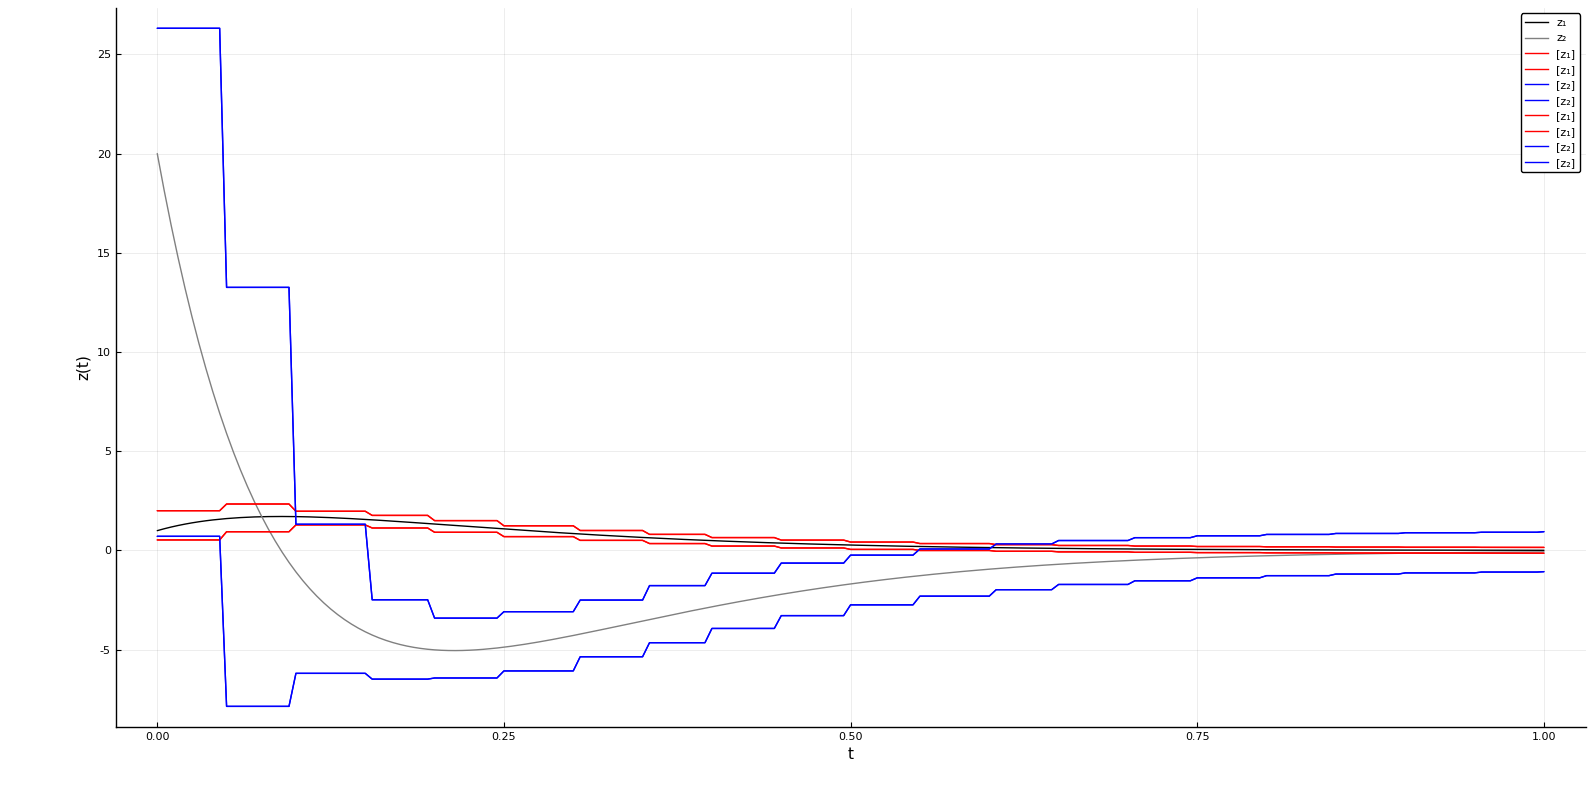
\includegraphics[width=1.0\textwidth]{fixedpoint_x.png}

\end{frame}

\begin{frame}[fragile]
    \frametitle{Step 1: for each $j = 1,\ldots$, priori enclosures}
    \framesubtitle{example: damped oscillator}
    
\begin{Verbatim}[fontsize=\small]
f(z::Vector) = [0 1; -64 -16] * z
Jz(t::Real) = [exp(-8*t) + 8*t*exp(-8*t)   t*exp(-8*t);
               -64*t*exp(-8*t)   exp(-8*t) - 8*t*exp(-8*t)]
\end{Verbatim}

    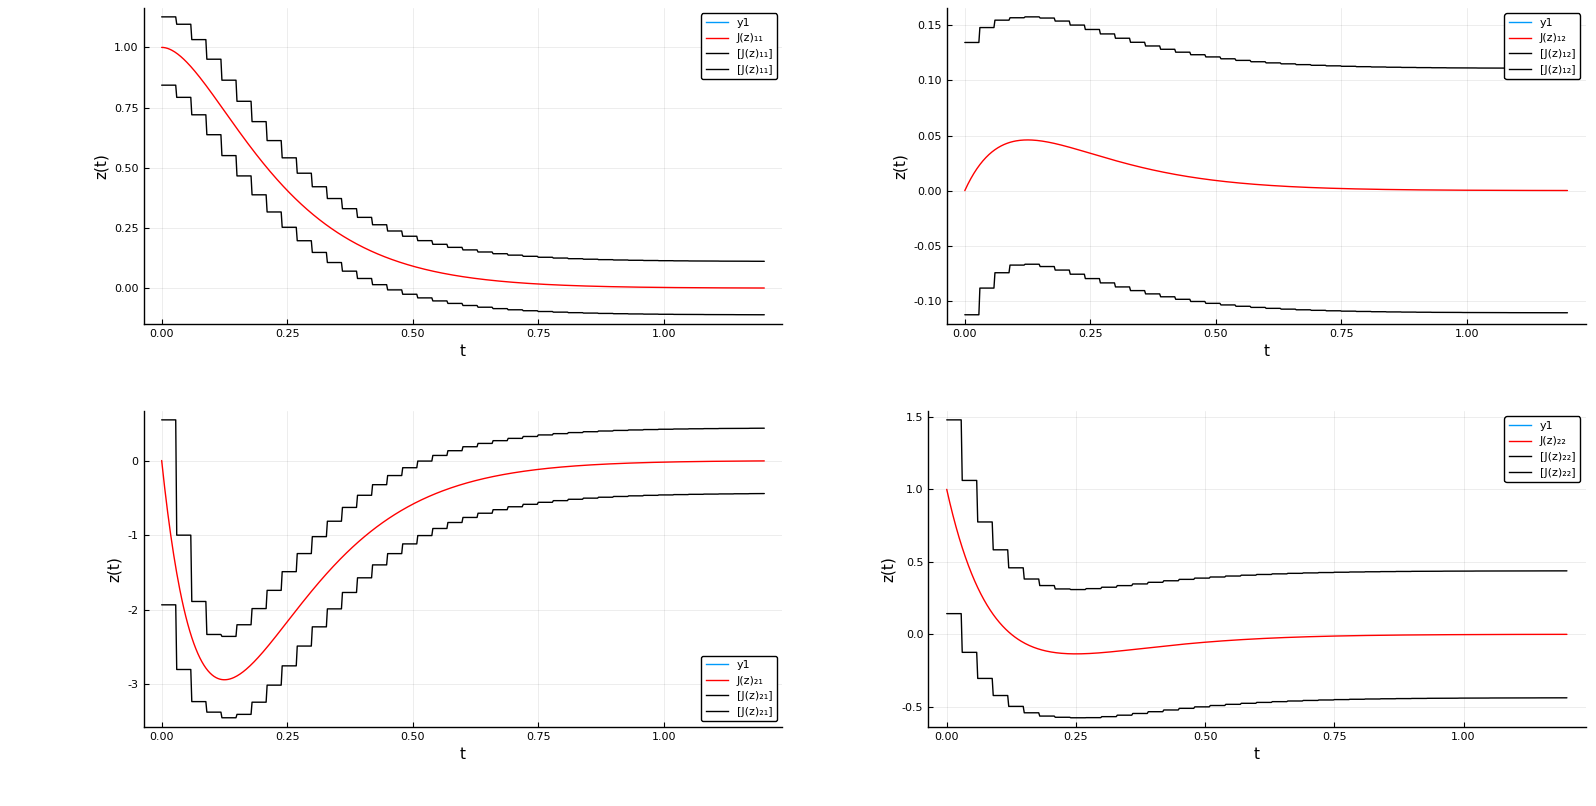
\includegraphics[width=1.0\textwidth]{fixedpoint_J.png}

\end{frame}

\note{
    One thing outstanding is to compare the priori enclosures calculated in Flowpipes.jl against the ones calculated by RINO.
    Sometimes the priori enclosure are ill fitting as you can see in this case.
}

\begin{frame}
    \frametitle{Step 2: for each $j = 1,\ldots$, taylor approximations}

    Get taylor outer approximations $[\bm{x}](t_{j+1}, t_j, \intervalbox{j})$, 
    $[\bm{x}](t_{j+1}, t_j, \tintervalbox{j})$ 
    and $[J](t_{j+1}, t_j, \intervalbox{j})$

\end{frame}

\begin{frame}
    \frametitle{Step 2: for each $j = 1,\ldots$, taylor approximations}
    \framesubtitle{Automatic generation of taylor coefficients}

    \begin{equation}
        J(\bm{f}) = \bmat
            \frac{\partial f_1}{\partial x_1} & \cdots & \frac{\partial f_1}{\partial x_n} \\
            \vdots & & \vdots \\
            \frac{\partial f_n}{\partial x_1} & \cdots & \frac{\partial f_n}{\partial x_n}
        \emat
    \end{equation}

    $\autof{1} = \bm{f}$
    
    $\autof{i+1} = J(\autof{i}) \cdot \bm{f}$
    
    \vspace{3mm}
    $\dot{\bm{x}} = \bm{f}(\bm{x})$ has the solution for some $\zeta \in [t_0, t]$
    $$\bm{x}(t, t_0, \iterx{0}) = \iterx{0} + \sum^{k-1}_{i=1} \frac{(t - t_0)^i}{i!} \autof{i}(\iterx{0}) + \frac{(t - t_0)^k}{k!} \autof{k}(\bm{x}(\zeta))$$

\end{frame}

\note{
    The authors of the paper took most of these steps (sub-procedures from) N. S. Nedialkov. Someone who extended DE problems to intervals. This is another one of those sub-procedures.
    The error term at the very end is the Lagrange expression of the error.

    $\set{ \bm{x}(t, t_j, \intervalbox{j}) : t \in [t_j, t_{j+1}] } \subseteq \enclosure{j+1}$
    Means that we can just replace $\bm{\zeta}$ with the priori enclosure.

    This expression can be extrapolated to have interval values so that we can outer bound the $k$-th order taylor approximation of the solution.
}

\begin{frame}
    \frametitle{Step 2: for each $j = 1,\ldots$, taylor approximations}

    \begin{multline*}
        [\bm{x}](t, t_j, \intervalbox{j}) = \intervalbox{j} + \sum^{k-1}_{i=1} \frac{(t - t_j)^i}{i!} \autof{i}(\intervalbox{j}) \\
    + \frac{(t - t_j)^k}{k!} \autof{k}(\enclosure{j+1})
    \end{multline*}
    
    \begin{multline*}
        [J](t, t_j, \Intervalbox{j}) = \Intervalbox{j} + \sum^{k-1}_{i=1} \frac{(t - t_j)^i}{i!} \Jac{\bm{x}} \autof{i}(\intervalbox{j}) \Intervalbox{j} \\
        + \frac{(t - t_j)^k}{k!} \Jac{\bm{x}} \autof{k}(\enclosure{j+1}) \Enclosure{j+1}
    \end{multline*}

\end{frame}

\note{
    I won't go into how the taylor approximation of the jacobian works for time.
}

\begin{frame}[fragile]
    \frametitle{Step 2: for each $j = 1,\ldots$, taylor approximations}
    \framesubtitle{example: damped oscillator}
    
\begin{verbatim}
f(z::Vector) = [0 1; -64 -16] * z
z(t::Real) = exp(-8*t)*[1 + 28*t; 20 - 224*t]
\end{verbatim}

    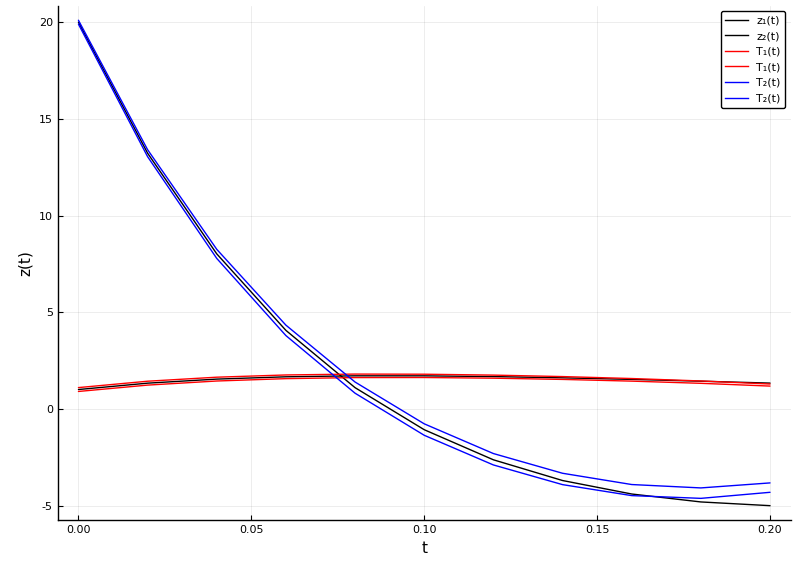
\includegraphics[width=0.9\textheight]{affine_tm_x.png}

\end{frame}

\begin{frame}[fragile]
    \frametitle{Step 1: for each $j = 1,\ldots$, priori enclosures}
    \framesubtitle{example: damped oscillator}
    
\begin{Verbatim}[fontsize=\small]
f(z::Vector) = [0 1; -64 -16] * z
Jz(t::Real) = [exp(-8*t) + 8*t*exp(-8*t)   t*exp(-8*t);
               -64*t*exp(-8*t)   exp(-8*t) - 8*t*exp(-8*t)]
\end{Verbatim}

    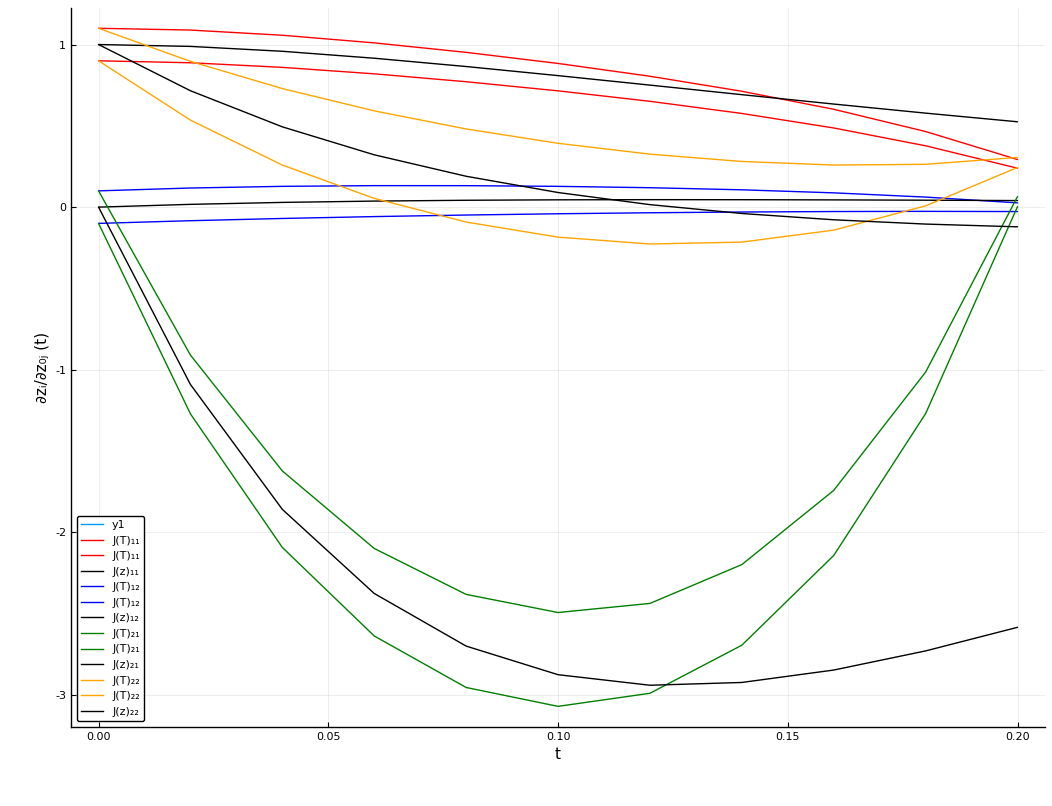
\includegraphics[width=0.9\textheight]{affine_tm_J.png}

\end{frame}

\begin{frame}
    \frametitle{Step 3: for each $j = 1,\ldots$, inner approximation}

    Deduce an inner approximation $]\bm{x}[(t_{j+1}, t_j)$

\end{frame}

\begin{frame}
    \frametitle{Step 3: for each $j = 1,\ldots$, inner approximation}
    \framesubtitle{Mean-value AE-extension}

    Let $f: \Reals^n \ra \Reals$, $[\bm{x}] \in \RIntervals^n$, $\tilde{x} \in [\bm{x}]$
    
    and $\bm{\Delta} \in \RIntervals^n$ such that $\set{\frac{\partial f}{\partial x_i}(x) : x \in [\bm{x}]} \subseteq \Delta_i$.
    
    \vspace{7mm}
    If $]\bm{z}[ \; = f(\tilde{x}) + \bm{\Delta}(\dual \; [\bm{x}] - \tilde{x})$ is an improper integral vector, then
 
    \vspace{7mm}
    $(\forall z \in \; ]z[) (\exists \bm{x} \in [\bm{x}]) (f(\bm{x}) = z)$
    making $\dual \; ]z[$ an inner approximation

\end{frame}

\note{
    This is the only step where we are utilizing modal intervals.
    
    I went over the mean-value AE extension in my last presentation and you may not remember it anymore, but for the sake of time I'll just mention the one important result I use, which is the calculation of $]\bm{z}[$.
    It's not neccessary for the result $]\bm{z}[$ to be an improper integral vector, but if it is (all of the vector components are improper integrals) then $]\bm{z}[$ is an inner approximation.
}

\begin{frame}
    \frametitle{Step 3: for each $j = 1,\ldots$, inner approximation}

    Define:

    $]\bm{x}[(t, t_j) := [\bm{x}](t, t_j, \tintervalbox{j}) + [\bm{J}](t, t_j, \intervalbox{j})(\dual\intervalbox{0} - \tilde{\bm{x}}^{(0)})$

    \vspace{2mm}
    If it is improper for given $t$, then $\dual \; ]\bm{x}[(t, t_j)$ is an inner approximation.

\end{frame}

\note{
    Therefore we can express a formula of possibly obtaining inner approximation $]\bm{x}[$ using the mean value AE-extension for the solution $\bm{x}$ using the outer bound of the taylor approximations of $\bm{x}$ and $\bm{x}$ we found earlier.

    Recall $\tilde{\bm{x}}^{(j)}$ is the approximation of the center of the inputs at iteration $j$.
}

\begin{frame}
    \frametitle{Step 4: for each $j = 1,\ldots$, set up next step}

    Set $]\iterx{j+1}[$, $\intervalbox{j+1}, \tintervalbox{j+1}$ and $\Intervalbox{j+1}$

    \vspace{7mm}
    $]\iterx{j+1}[ \quad = \quad ]\bm{x}[(t_{j+1}, t_j)$
    
    \vspace{3mm}
    $\intervalbox{j+1} = [\bm{x}](t_{j+1}, t_j, \intervalbox{j})$

    \vspace{3mm}
    $\tintervalbox{j+1} = [\bm{x}](t_{j+1}, t_j, \tintervalbox{j})$

    \vspace{3mm}
    $\Intervalbox{j+1} = [J](t_{j+1}, t_j, \intervalbox{j})$

\end{frame}

\note{
    Now we've done iteration $j$ and we can set up the interval boxes for iteration $j+1$ and repeat.

    So what does the Flowpipes.jl implementation give us? In the next slide I have a plot of the inner/outer approx. for a specific problem.
}

\begin{frame}[fragile]
    \frametitle{Solution: Flowpipes.jl algorithm}
    \framesubtitle{example: Brusselator}

\begin{verbatim}
f(z::Vector) = [1.0 - 2.5*z[1] + z[2]*z[1]^2;
    1.5*z[1] - z[2]*z[1]^2]
\end{verbatim}

    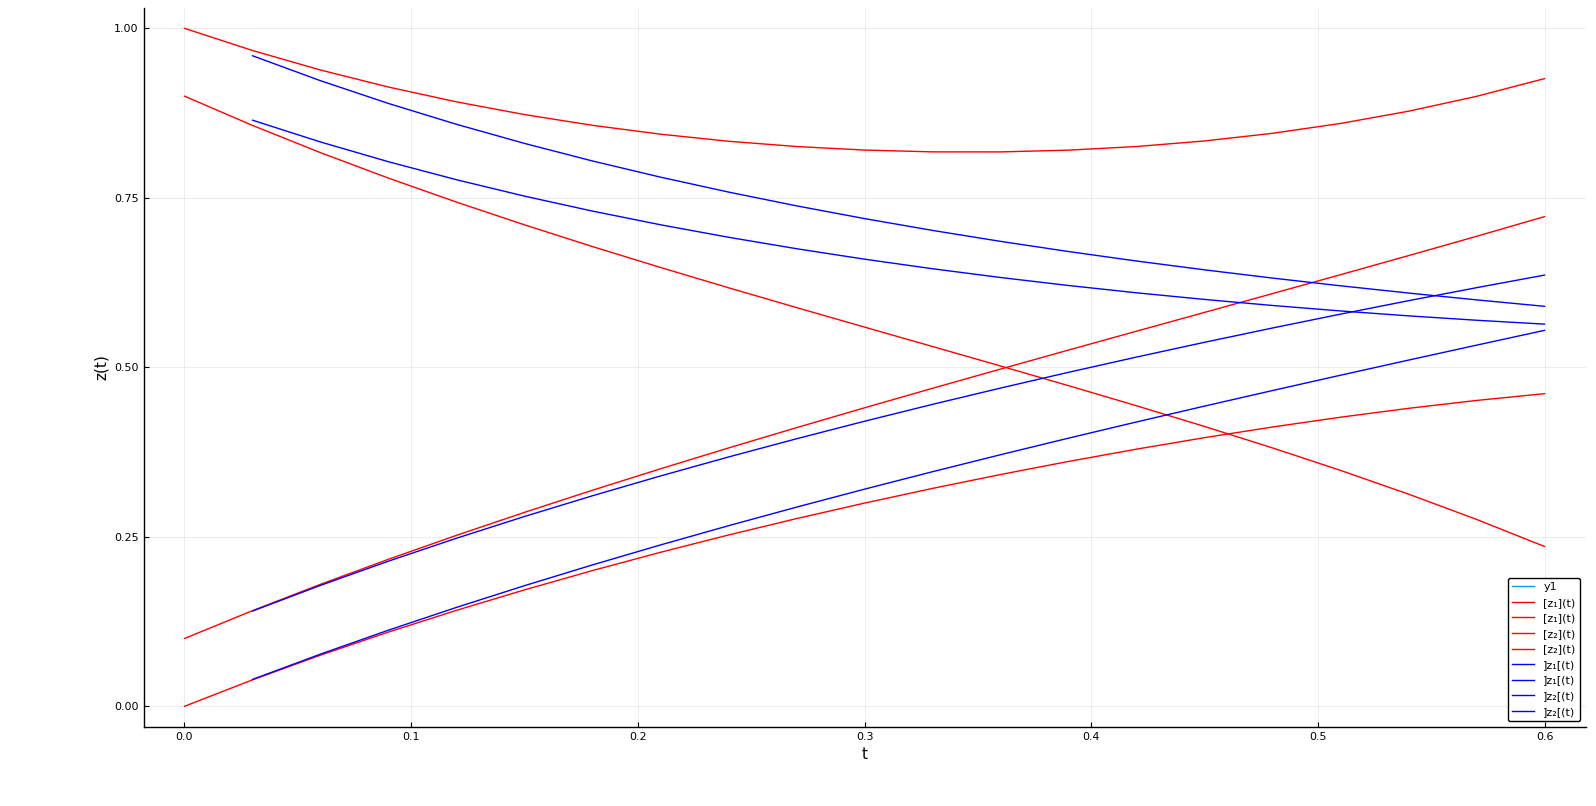
\includegraphics[width=1.0\textwidth]{brusselator_short.png}

\end{frame}

\note{
    Well that is quite underwhelming. We have the inner/outer approx. of the flowpipe but it breaks apart in $t_n = 1$.
While this result is better than simply using taylor approximations strictly, the inner approximation shrinks and the outer approximation expands.
}

\begin{frame}[fragile]
    \frametitle{Solution: Flowpipes.jl algorithm}
    \framesubtitle{example: Brusselator}

\begin{verbatim}
f(z::Vector) = [1.0 - 2.5*z[1] + z[2]*z[1]^2;
    1.5*z[1] - z[2]*z[1]^2]
\end{verbatim}

    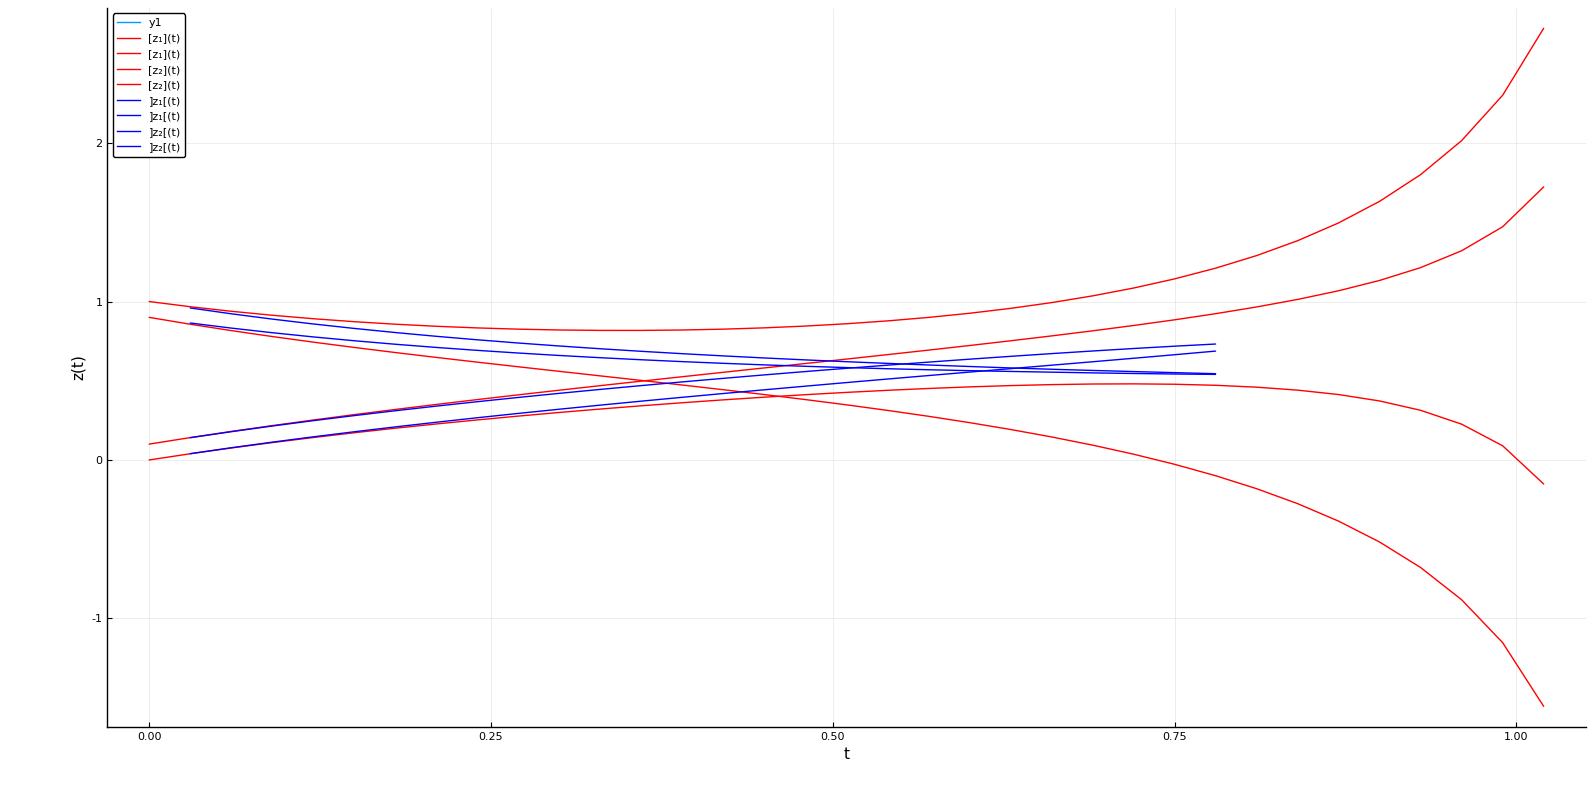
\includegraphics[width=1.0\textwidth]{brusselator_long.png}

\end{frame}

\begin{frame}
    \frametitle{Solution: Flowpipes.jl algorithm}
    \framesubtitle{example: Brusselator}

    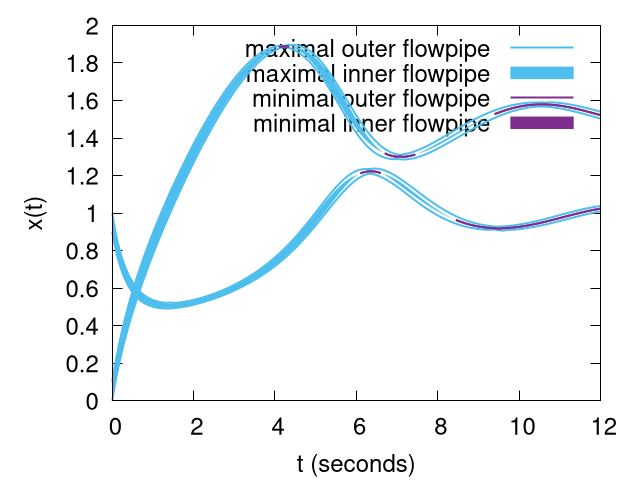
\includegraphics[width=1.0\textheight]{brusselator_compare.png}

\end{frame}

\note{
    Comparing that with the RINO C++ implementation it's clear RINO's much better since the flowpipe approx. last even after $t = 12$.
}

\begin{frame}[fragile]
    \frametitle{Solution: Flowpipes.jl algorithm}
    \framesubtitle{example: damped oscillator}

\begin{verbatim}
f(z::Vector) = [0 1; -64 -16] * z
z(t::Real) = exp(-8*t)*[1 + 28*t; 20 - 224*t]
\end{verbatim}

    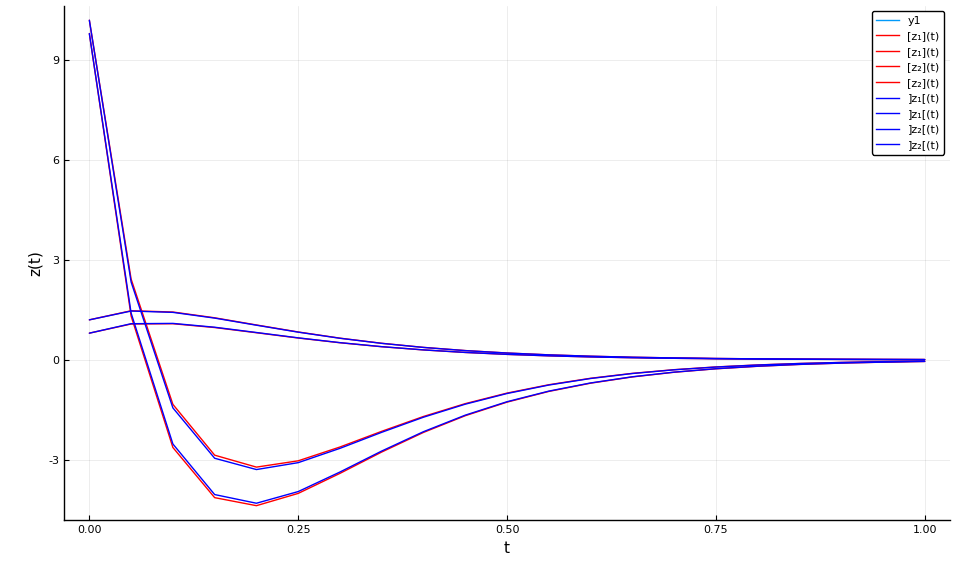
\includegraphics[width=1.0\textheight]{oscillator.png}

\end{frame}

\note{
    For problems with analytical solution Flowpipes.jl gives quite accurate results. So I'm not sure what is making Flowpipes.jl give bad approximations for the Brusselator and some other problems.
}

\begin{frame}
    \frametitle{Solution: Flowpipes.jl}

    \vspace{5mm}
    \begin{enumerate}
        \item Flowpipes.jl
        \item AffineArithmetic.jl (better intervals)
        \item ModalIntervalArithmetic.jl
        \item hacked ForwardDiff.jl
    \end{enumerate}

    \vspace{5mm}
    Things to do: do away with \texttt{ForwardDiff.jacobian(f, x)}, Zygote.jl, ???

    \vspace{5mm}
    \url{https://github.com/fireofearth/2019s-verification}

\end{frame}

\note{
    Two problems with Flowpipes.jl is

    1. Appoximations are really bad.

    2. The algorithm is also very slow. RINO calculates inner/outer appoximations over $[0, 12]$ almost instantaneously whereas Flowpipes.jl takes minutes to calculate over $[0, 1]$.

I rely on ForwardDiff.jl. It does not directly compute taylor coefficients for taylor solutions of ODEs. It does not directly compute higher order derivatives.
I have to compose taylor coefficients by applying ForwardDiff.jacobian(f, x) over and over again using a loop.

Higher order derivatives take a drastically long time to compute, and is not set up for inputs that are interval or affine.
Additionally ForwardDiff.jl does not use source code transformation (SCT), and uses operator overloading (OO) and dual numbers instead. We may high runtime complexity for operations on hyper-dual numbers while doing higher order derivatives.
}

\end{document}
